\section{FAB-MAP 2.0}

\subsection{Introduction}
\begin{frame}{FAB-MAP 2.0}
    \begin{itemize}
        \item What happened after version 1.0 ?
    \end{itemize}
    \begin{quotation}
        We describe a formulation which preserves almost all the key features of our earlier model, but allows for the exploitation of the sparsity of visual word data to achieve large reductions in computation and memory requirements.~\cite{fabmap2011}
    \end{quotation}
    \begin{itemize}
        \item General intuition of the work in 2.0
            %\begin{itemize}
                %\item Multiple changes for scalability
            %\end{itemize}
    \end{itemize}
    \note[item]{Read quotation}
    \note[item]{I will not go into details... General intuition/main points.}
\end{frame}

\subsection{Modifications}
\begin{frame}
    \frametitle{Modifications}
    \begin{itemize}
        \item Sparse approximation
        \item Inverted index
        \item Appearance likelihood changed in two ways
            \begin{enumerate}
                \item Negative observations greatly outnumber positive ones, and are also generally less informative.
                \item Data association
            \end{enumerate}
        \item Implementation in O(\#vocab)
    \end{itemize}
    \note[item]{Sparse approx of the to the FAB-MAP model}
    \note[item]{Implementation using inverted index... What is it ?}
    \note[item]{If a document is considered as a list of word identifiers, then an inverted index maintains the inverse mapping from words to documents.}
    \note[item]{Appearance likelihood was changed in two ways to work with inverted index}
    \note[item]{*Single* probabilistic term for all observations of a place. Lead to some (negligible) information lost}
    \note[item]{Data association: sample-based instead of average appearance of a location (Location == set of samples.... Better suited for multi-modal)}
    \note[item]{They give the example of the open vs closed door}
\end{frame}

\subsection{Modifications}
\begin{frame}{Geometric Verification}
    \begin{itemize}
        \item add geometric verification(100 most likely samples) (essential at large scale)... add a figure to show what it is
    \end{itemize}
    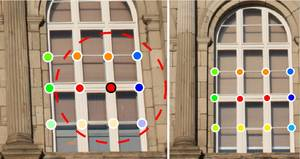
\includegraphics[width=1.0\textwidth]{./media/geo_verif.jpg}
\end{frame}

\begin{frame}{K-Means}
    \begin{itemize}
        \item Approx algo of k-means
        \item To avoid these effects, we choose the initial cluster centers for k-means using a fixed-radius incremental pre-clustering, where the data points are inspected sequentially, and a new cluster center is initialized for every data point that lies further than a fixed threshold from all existing clusters. This is similar to the furthest-first initialization technique (Dasgupta and Long 2005), but more computation-ally tractable for large data sets. (show figure 6,7)
        \item We also modify k-means by adding a cluster merging heuristic. After each k-means iteration, if any two cluster centers are closer than a fixed threshold, one of the two cluster centers is re-initialized to a random location.
        \item This boosted performance of the system
    \end{itemize}
    \note[item]{To maintain system performance at scale, they had to make some changes}
\end{frame}

\begin{frame}{K-Means words}
    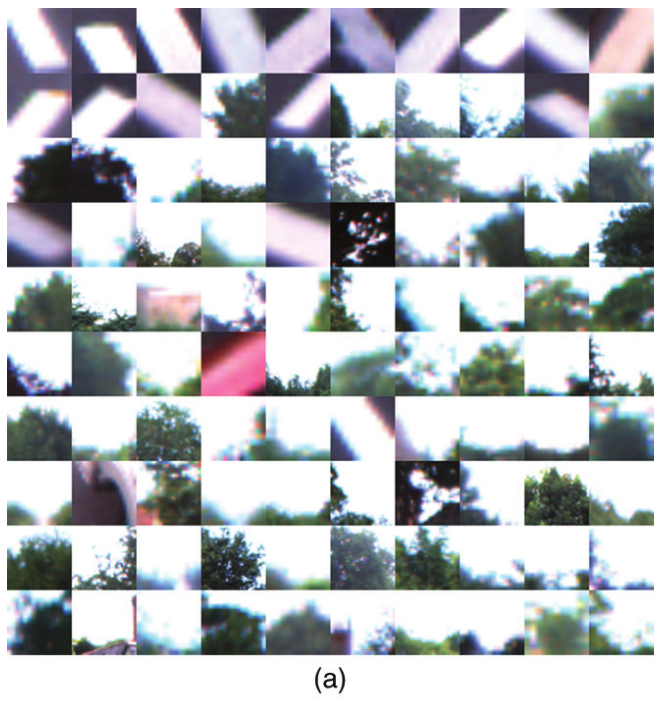
\includegraphics[width=0.5\textwidth]{./media/words_fabmap2a.png}
    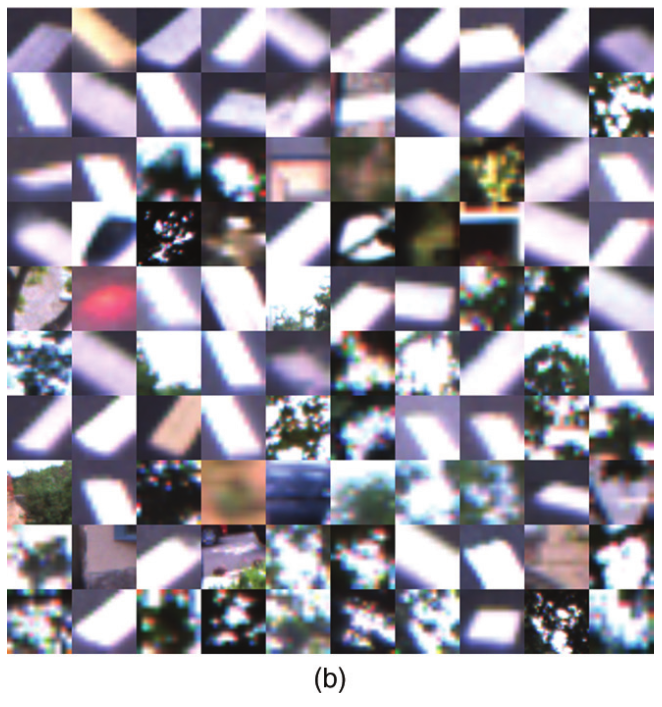
\includegraphics[width=0.5\textwidth]{./media/words_fabmap2b.png}
\end{frame}

\begin{frame}[t]{K-Means Precision-Recall}
    \begin{center}
        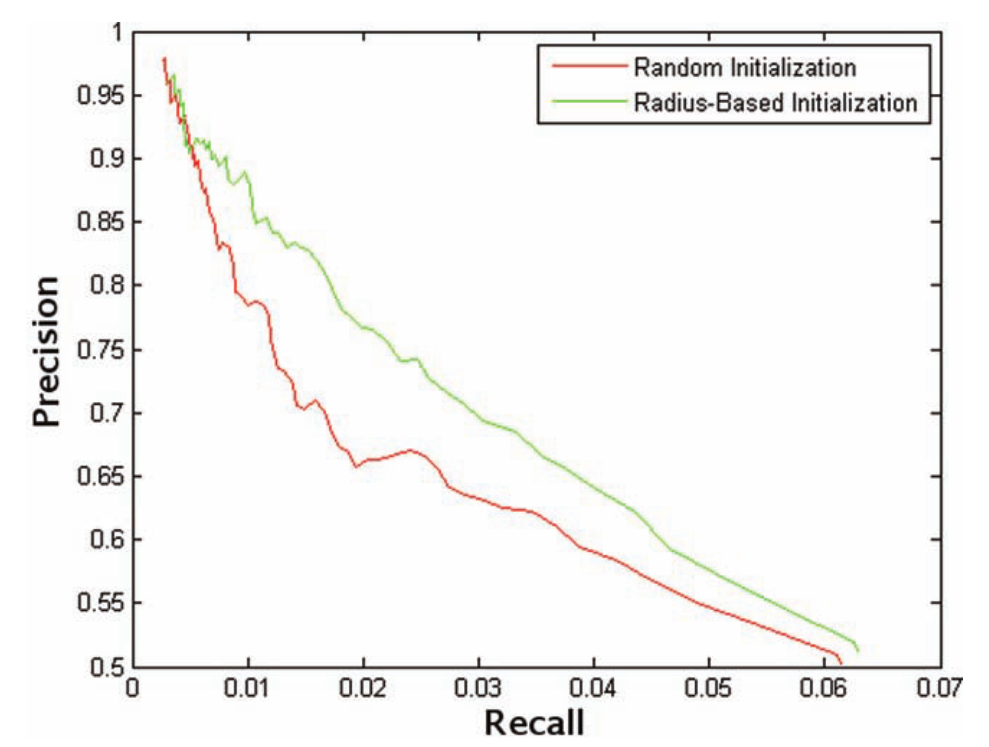
\includegraphics[width=0.7\textwidth]{./media/precision_recall_kmeans.png}
    \end{center}
\end{frame}

\subsection{Results}
\begin{frame}
    \frametitle{Results}
    \begin{itemize}
        \item validate the work on a 1000km data set; (show the SLAM figure)... Really aimed at large scale (other with 66km but they have the biggest)
        \item 1000 km data, compared with tf-idf ranking measurements
        \item Ground thruth = GPS, correct match less than 40m... A bit relax (89\% were separated by less than 5 m, and 98\% by less than 10m)
        \item Add result Figure 11
        \item Maybe table 3, indicate that CL vs NB for 100\% precision
        \item 14ms filter update + geo check, 423ms for SURF, 60ms Quantization
        \item 4400 times faster than 1.0, spase representation lead to O(1) instead of O(\#vocab)
    \end{itemize}
\end{frame}

%%%%%%%%%%%%%%%%%%%%%%%%%%%%%%%%%%%%%%%%%%%%%%%%%%%%%%%%%%%%%%%%%%%%%%%%%%%%%%%%

\begin{frame}
    \frametitle{FAB-MAP 2.0}
    At time k, our map of the environment is a collection of nk discrete and disjoint locations Lk = ?L1, ... ,Lnk ?. Each of these locations has an associated appearance model, which we parameterize in terms of unobservable ‘scene elements’, eq. A detector, D, yields visual word observations which are noisy measurements of the existence of the under- lying scene element eq. The appearance model of a location in the map is our belief about the existence of each scene element at that location:
\end{frame}

